\documentclass[a4paper, 12pt]{article}

\usepackage[utf8]{inputenc}
\usepackage[T2A]{fontenc}
\usepackage[english,russian]{babel}

\usepackage{cmap}
\usepackage{calc}
\usepackage{enumitem}
\setlist{nolistsep}
\usepackage{mathtext,mathtools,amsmath,amssymb}
\usepackage{xcolor}
\definecolor{allrefs}{HTML}{1010aa}
\usepackage[
	linktoc=page,
	colorlinks=true,
	allcolors=allrefs
]{hyperref}

\frenchspacing
\linespread{1.3}
\usepackage{indentfirst}
%\setlength{\parindent}{10pt}
\usepackage{graphicx}
\usepackage[multidot]{grffile}
\usepackage[labelsep=period]{caption}
\makeatletter
\g@addto@macro\@floatboxreset\centering
\makeatother

\usepackage[
	vmargin=1in,
	hmargin=1in
]{geometry}
\usepackage{multicol}
\usepackage{cuted}
\setlength{\columnsep}{.25in}
\usepackage{flushend}

\def\datee#1{\hfill\textbf{#1} \par}
\def\mailto#1{\href{mailto:#1}{#1}}


\begin{document}

\thispagestyle{empty}
\noindent 
Юлия Игоревна Лащинская 
\hfill
\mailto{lashinskaya.iulia@yandex.ru}
\\

\vfill

\begin{center}
\Large\bf
Экономика
\end{center}

Обычно на лекциях дается вопрос. На каких-то лекциях будет задание на дом, ответить на вопрос, найти в инете, повторить что было на лекции, сдавать домашки в бумажном виде на лекции. По результатам летучек и этих домашек может быть автомат. 

\vfill

\begin{center}
2020
\end{center}

\clearpage
\tableofcontents
\clearpage


\section{Предпринимательство}

\subsection{Предприниматели}

%%%%%%%%%%%%%%
\datee{Feb 12}

На почту отправят информацию о курсе. 10\% людей склонны к предпринимательству. А почему у одних получается и вообще возникает это дело само собой, а у других не выходит ни при каких обстоятельствах? Мелкое и инновационное предпринимательство (старт ап). Возникновение креативного класса в противоположность доминированию сфере услуг. Говорили, что сельскохозяйственное общество? потом индустриальное, потом в сфере услуг преобладание численности. Почему Америка является доминантом в сфере стартапов и малого бизнеса, почему она первоначальник и какие там условия по сравнению с Европой и нами. 

Предприниматели. Важное понятие риск, всегда связано с предпринимателем. Вот есть страхование чего-угодно, оно связано с потребностью избавиться от рисков. Предприниматель сознательно идет на риск, и для него это не бравада, что вот я риск преодолею, а сам процесс участия в риске и выход успешный из него подстегивает на предпринимательство. Специально ищутся такие ситуации. Идя на риск, предприниматель еще и дает обществу всякие вещи. И изобретения тоже давались естественно с трудом, внедрение их тоже. Но вопрос -- почему не у всех такое отношение к риску? Некоторые исследователи рассматривали с точки зрения особенностей организма: у каждого по-своему устроена нервная система, считается, что есть группа людей с выделяющейся симпатической нервной системой, при возбуждении которой снимается мышечное утомление, люди могут долго работать без усталости. У людей с активным этим отделом по-другому устроены некоторые ткани и скорости хим реакций, и люди нуждаются в воздействии этой части нервной системы, в их раздражении. В пиковых ситуациях выбрасывается адреналин, человек чувствует, что любая цель достижима и так далее. Такая же ситуация возникает и при опьянении, но это чувство временное, нельзя сказать, что оно действительно приведет к правильному выходу из возбуждающей ситуации, нужно, чтобы человек ощущал уверенность в себе, что разрешит ситуацию. Например есть спокойные водители, а есть те, кто нервничает, они водят плохо. Предприниматель не думает вот как бы мне отсюда выйти из ситуации, хоть бы что-то не случилось. Предприниматель уверен, что он найдет выход обязательно. Чувство надежности определяется содержанием эндорфинов и других гормонов, которые схожи с морфием по действию. Другие тормозящие нервную систему вещества все-таки подавляют некоторые реакции, а если в крови есть, организм сам по себе делает и поддерживает. Отсюда можно перейти к вопросу о наследниках. Часто дети, особенно уже к третьему поколению, люди не особо хорошо делают это дело. 

У любого человека есть противоречие между тем, что надо делать, и тем, что хочется. У предпринимателей и творческих людей не возникает такого противоречия, присутствует живой интерес к делу. Экономисты (Йозеф Шумпетер) разделяют предпринимателей и бизнесменов, предприниматель отождествляет себя с делом, а бизнесмен с капиталом. Пусть есть играющий на фондовом рынкам и есть банкир, у них очень высокая прибыль, но интересна ли такая работа, у них важно получить побольше денег и иметь меньше рисков. А предприниматель все время ищет достаточно хороший товар, ему важна содержательная сторона занятия. Не всегда вознаграждение для предпринимателя главное. Шульпетер говорил, что это способность взять риск, это инновации, не только продукт, но и бизнес модель новая может быть, это соединение всех факторов производства (труд, земля, капитал), умение их подобрать. Три мотива предпринимателей: потребность в господстве, власти и влиянии (не потерпит работать под чьим-то руководством, предприниматель не может подчиняться косности и консервативности), жажда победы над соперником и над собой, жажда творчества. 

В Америке в Школу Бизнеса Гарварда принимают прошедших тест на предпринимателя, тест Мейерса-Бриггса. 83\% выпускников остаются предпринимателями не менее 5 лет. Попытались для эксперимента принять человек, не прошедших тест, но хотящих учиться, из них только 28\%. Гарвардский медицинский центр заключил, что только 1\% обладает исключительной творческой потенцией предпринимательства, 10\% нормально подходят для предпринимательства, 60\% имеют какие-то такие случайные элементы, а 30\% вообще не способны. 

\subsection{Инновации}

Теперь об инновациях. Шумпетер считал, что инновация не может состояться, если новая точка равновесия расположена близко к старой. Исследователи писали, что инновация это новые способы работы, новые продукты, новые способы управления компанией. Инновация это не наука о дисциплине, там нет никакого консерватизма. Неправильный ответ не исключается, поскольку может привести к правильному решению. Большому бизнесу перемены особо не выгодны, никакие чиновники и подобные товарищи тоже не хотят. Новаторы не могут жить в крупном устойчивом бизнесе. Инновации не возникают сами по себе, их появление нужно мотивировать и поддерживать. Например, Дисней проводит три раза в год конкурс на новые идеи. Гугл предоставляет техническим специалистам один день для предложения бизнес идей. Найк практикует поездки за новыми идеями для менеджеров и прочих, они общаются со спортсменами, иногда сами потребители подсказывают. Майкрософт каждые 7 лет дает год на творческий отпуск. В Японии тоже куча идей, в Сони стараются увлечь потребителя, совершенствуя свою продукцию, они считают, что потребители часто не знают что хотят или даже не знают, на что производители способны. 

Теперь про методы мышления. 16 навыков выделяют новатора от стандартного стиля мышления. 
\begin{enumerate}
\item Многоэкранное мышление вместо узкофокусного. Обычный человек, решая проблему, смотрит только на нее саму и забывает среду вокруг нее. А взаимодействие со средой могут помочь в решении. Не умея так подходить к вопросу, нормально проблему не решить. 
\item Прорывное мышление против компромиссного. Старые методы могут не подходить. Например, надо увеличить количество продаж, обычно можно было бы увеличить штат, число точек продажи, будут прибыль и затраты. 
\item Абстрактное мышление против специализированного. Когда мы концентрируемся на конкретном объекте, он часто связан со стереотипами, мы не можем увидеть аналогии с другими областями жизни. По аналогиям можно часто найти ответ или подсказку. 
\item Радикальное обострение требований при постановке задачи. Телефон стационарный часто не используется дома, но десятки лет назад если б какому-то разработчику сказали создать маленький мобильный телефон, он бы вообде
\item Нелинейное мышление против линейного. Ни один прогноз как правило не сбывается, долгосрочные особенно. Происходит так потому что предсказание не учитывает все переходы. У новатора задача интуитивно почувствовать все преобразования. 
\item Многообразное вместо узкоспециализированного. Эйнштейн и Томас Эддисон держали по 8 и 10 тысяч книг дома. 
\item Ресурсное против затратного. Вот вам больше денег вложим и посмотрим что будет. Вот в Москве вложишь, их своруют и еще и попросят еще. А вдали в России люди понимают, что это их регион, и вообще нужно трудиться, они ухитряются на несколько направлений потратить, размещают рационально. 
\item Функционально ориентированное против объектно ориентированного. Потребность выпить хороший кофе, люди выдумывают кофе машину, кофеварку, люди модернизируют эти объекты. И люди начинают модернизировать их. Но изначальная идея же была выпить кофе, а не модернизировать. 
\item Эволюционное мышление против случайного. Есть люди, не знающие законов развития например, развертывания пика свертывания, издержек. Незнание тормозит.
\item Долгосрочное мышление вместо краткосрочного. Краткосрочное обычно компромиссное. 
\item Аналитическое мышление против прыжкового. Эйнштейн говорил, что если бы имел час на решение задачи, потратил бы 55 минут на обдумывание и 5 на решение. 
\item Структурированное против стохастического. Имеется в виду мозговой штурм. В рекламе какой-то штурм возможен, но при создании спутника или инновации можно такой вред нанести всему сообществу. 
\item Творческое против призывного. НАСА проводила исследование, в каком возрасте больше всего развито творческое мышление. В результате чисто творчески мыслящих сильно сокращается с возрастом, с 98\% в 3--5 лет до 2\% во взрослой жизни. 
\item Умение видеть проблему. Компания долго работала над совершенствованием моющих средств, не знала как избавиться от катышков от тряпки, компания искала в химии решение, они обратились к дизайнерской фирме, которая вдруг нашла способ. Перемешивание пыли с водой приводит к катышкам, они придумали щетку такую, чтобы вода не попадала непосредственно к пыли. 
\item Конкретная цель вместо обобщенной. 
\item Потоковое мышление вместо одноразового. Генри Форд хотел создать автомобиль для всех, на него смотрели как на чудака. Но вопрос был еще и в дорогах, не особо было где ездить. Задумываясь об этом, сначала решали проблему с дорогами. 
\end{enumerate}

\subsection{Стартапы}

Стартапы. Термин появился в конце 70х, Форбс определил так компании с короткими циклами. Стартап, в отличие от малого бизнеса, рассчитан на быструю реализацию, потому что новую идею необходимо быстро осуществлять, потому что могут украсть. Дальше об особенностях: инновации, низкий уровень первоначальных вложений, потому что это неизбежность, быстрый рост, безысходный конец, маленький процент выживаемости. Критерии сравнения. Масштабы, для стартапы это стремление развиться в лидера рынка, желаемая трансформация в крупное предприятие, для малого бизнеса масштаб небольшой, связано с тем, что сама специфика не предполагает больших размеров, потому что это запрещает гибкость. Инновации, малый бизнес редко создает что-то уникальное. Активы, для малого бизнеса выделяют помещение, оборудование, для стартапа это интеллектуальная собственность. Прибыль, малый бизнес не может позволить себе работать без прибыли, потому что рост особо сильный не предполагается, у стартапа так можно, потому что необходим рост. Риск, у малого бизнеса можно оценить, у стартапа невозможно. 

Стадии развития стартапа. 
\begin{itemize}
\item Предпосевная. Существует только идея у основателя, можно еще продумать состав. 
\item Посевная. Анализ рынка, аудитории, на которую рассчитываешь. Формирование бизнес плана. SWOT analysis -- strengths weaknesses opportunities threats, нужно провести анализ всего этого на посевной стадии. Прописать какой уровень дохода ожидается через год. Источники финансирования могут быть семья, друзья, или бизнес ангел. Бизнес ангелы. этот термин пришел из Бродвея, обозначал спонсоров, финансировавших спектакль на благотворительной основе, но если оказывалось удачным, брали часть прибыли. Правительство США в 62 году выдвинуло задачу создания больших ЭВМ в рамках гонки вооружений, освоения космоса. В 62 году правительство финансировало все целиком, но к 69 году уже только 30\%, а потом всего 10\%. Тогда и появилось такое применение бизнес ангелов. Интерес бизнес ангела в том, что он конечно предприниматель, но ему уже не интересно так заниматься своим делом, а помогать и привнести свои навыки предпринимательские туда. Он не просто инвестор. Помогает, например, готовы копаться в мусоре для поиска по-настоящему хороших и прибыльных идей. Главная задача в минимизации риска. Они большее трезво смотрят и помогают выделить основателю стартапа хорошие вещи и слишком рисковые. Оценка полноценности команды, может даже привести свою команду. Использует свои связи для получения конкурентных и мнимых преимуществ при работе с клиентами. Мнимые это временные, но они важны на начале проекта. В среднем около 250к долларов бизнес ангел может выделить на посевной стадии. 
\item Создание прототипа. Прототип здесь означает предложение модели с минимальными характеристиками. Это еще модель, не представлена для пробирования. 
\item Разные версии продукта. Альфа версия создается по требованиям технического задания, но она не прошла технические тесты. Бета версия в двух вариантах, закрытая отличается тем, что продукт проходит ряд закрытых тестов, выбирается аудитория, которая ждала продукт, эти люди разбираются и могут однозначно одобрить, но таких людей может быть не слишком много. Потом начинается публичная бета версия, где аудитория выбирается случайно, и на основе отзывов этих людей совершенствуется продукт. 
\item Стадия стартапа. Значительно увеличиваются расходы. Бизнес ангелы могут дать денег вплоть до 2М долларов. Продукт производят в массовых количествах, главная задача -- показать инвесторам, что продукт перспективен. На этой стадии надо позаботиться о том, чтобы найти инвесторов. 
\item Стадия раннего роста. Наконец перешагиваем на точку безубыточности, наконец начинается рост. Вечурные фонды можно привлекать теперь. Это более крупные организации, чем бизнес ангелы. Это что-то вроде копилки, которая собирает средства разных инвесторов, организаций чаще всего, банки, пенсионные фонды, страховые компании. Вечурные фонды обязаны иметь хорошую прибыль, поэтому могут присоединиться только тут. 
\item Расширение. Вовсю участвуют эти фонды, можно привлечь банковские кредиты. До 100М долларов. 
\item Стадия выхода. Стадия выхода может быть и для бизнес ангела, и для основателя стартапа. Когда бизнес ангел вступал, он выбирал себе какую-то долю, иногда очень высокую, вплоть до 90\%. Выход означает выход на акционерное общество. Продав акции и получив прибыль, бизнес ангел уходит из этого дела и ищет новое. А основатели стартапа выходят часто потому что они творческие люди, а компания, которая становится крупной, теряет творческий потенциал. 
\end{itemize}


Америка сама себя считает самой пригодной для стартапов и малого бизнеса страной. Оказывается примерно 60\% Американских бизнесов имеет не более 4 сотрудников. На предприятиях размером менее 500 человек трудится более половины трудящихся. 70\% предпринимателей вложили менее 20к долларов, 14\% даже 1к. Основное сравнение с Японией, прежде всего относительно миграции. В Японии не так свободно разрешено, и поэтому типа в Японию способные люди не могут въезжать, а в Америку могут. Еще США богатая страна, это значит, что у людей много денег, и люди легко расстаются с деньгами в надежде еще разбогатеть. Гораздо легче добыть финансирование. Американские университеты лучшие в мире, при сравнении с Европой говорят, что концентрация ума по университетам более равномерное. В Америке лучшие преподаватели сосредоточены в конкретных вузах. Далее, в Америке работников можно легко увольнять, в Европе много бюрократических процедур социального характера. В Америке проще сформировать команду, потому что можно искать людей и увольнять неудачных без особой траты времени. В Америке вообще по-другому смотрят на найм, в Европе работа это особый статус, чем более стабильное место получил, тем престижнее для тебя это, в твоей среде вообще если тебя уволят, потеряешь много всего и станешь чуть ли не изгоем. В Японии с этим еще хуже. В Америке наоборот, если человек все время старается преодолевать трудности, уходит с работы не потому что что-то не получилось, а чтобы вырасти еще, больше уважения. Многие стартапы зарождались там, где это делать не совсем законно, например, в гаражах. В Европе бы на них донесли и все. Америка обладает большим внутренним рынком, это вызывает дополнительный спрос с мелких производителей. В Америке профессия выбирается динамически. В Европе склонность считать, что у человека всегда свое место, своя карьера и так далее, а в Америке возникает беспорядочность и быстро меняется рынок. Можно позаниматься чем-то одним, потом бросить и перейти к другому. Однако с примерно 70 годов Америка попала под финансовые что-то там. 


Ошибки организаторов стартапов и малого бизнеса. Часто мы думаем, что можно набрать легко кредиты и начать свое дело. Если набрал потребительских кредитов, а предпринимательство не сложилось, будет большая неудача. Собственный бизнес дарит людям свободу, думают люди, сам себе хозяин. Но нет, бизнес занимает все время, без выходных и прочего. Считается, что если тебе бизнес чисто для денег, ничего не выйдет, нужно все продумывать. Часто иллюзии, что клиентам обязательно потребуется что-то. Нужно не только начать, но и потом разрабатывать, трансформировать продукт для поддержания интереса. Чисто финансовая сторона -- мы часто вкладываем средства, не замечая, что никакой хорошей отдачи нет, нужно вовремя бросить дело, сохранив денег. На фондовом рынке особенно заметно, и в казино, новички не бросают вовремя. Найм своих друзей и членов семьи. Считается, что наверняка отношения между вами испортятся. Друзьями могут остаться люди, разрабатывавшие вместе это дело. 


\subsection{Креативный класс}

Ценность креативного класса очень высока. Например, появление каршеринга уменьшило статусность обладания авто. С жильем тоже, можно лишь снимать. Собственность теряет смысл. Прежде всего, креативный класс ценит индивидуальность, не считается с нормами. Милитократия, креативные профессионалы не идентифицируют себя по деньгам и месту в обществе. Если раньше был определенный дресс код, то теперь прийти на работу в джинсах и кедах нормально, потому что одевающийся так человек может иметь такие способности, что он выдвигает всю фирму сразу. И конечно не важно как он выглядит. И отсюда всякие однополые браки и подобное тоже не отвергаются. Пестрость ценна потому что у них может быть потенциал для создания продуктов и услуг. Тезис, что мы можем нанимать кого угодно без каких-то дискриминаций. Креативный класс хоть и не ценит, как говорят, зарплату, но почасовая зарплата у них самая высокая. Они ценят гибкие условия труда, чисто психологическое явление. Гибкий график необходим для того, чтобы пополнять свои творческие потенции. Люди занимаются какой-нибудь живописью, путешествиями (сейчас развивается из-за необходимости большего числа творческих людей). Гибкость это еще возможность влиять на свою обстановку и чтобы никто не давил. Признание со стороны коллег. Один человек дает интервью и говорит, что больше всего хочет уважения коллег, развлечением становится сама работа и наверно в этом вообще секрет энтузиазма. Горизонтальная гипермобильность. Американцы предпочитают быстро менять работу, в среднем 3.5 года. Между 20 и 30 годами вообще чуть больше года. IT сотрудники все работают уже на работе менее 4 лет и сменить хотят менее, чем через 3 года. Самоутверждение на каждом новом месте работы это похвала себе. 

\subsection{Доходы и расходы}

Важно три момента. Мы часто сталкиваемся с понятием рентабельность, но не всегда понимаем что это такое. Ценообразование не универсально, есть несколько методов, их не особо много, но несколько. Точку безубыточности нужно просчитывать всегда и старательно. 
Рентабельность
\begin{center}
\begin{tabular}{| l l |}
\hline
\multicolumn{2}{| c |}{\underline{Баланс}}\\
\ \hfill Активы \hfill\ & \ \hfill Пассивы \hfill \ \\
\hline 
Внеоборотные & Собственный капитал \\
Оборотные & \hfill уставной капитал, \\
- запасы & \hfill нераспр. прибыль\\ 
- дебеторская задолженность & Долгосрочные обязательства (>года)\\ 
\ \ -- то, что нам должны поставщики, & Краткосрочные (<года) \\
\ \  покупатели & \hfill как кредиты \\
- наши денежные средства & \\
\hline
\end{tabular}
\end{center}
%
%\begin{center}
%\begin{tabular}{| l | l | l | l | l |}
%\hline
%выручка & Прямые переменные расходы &&& \\
%\hline
%& маржинальная прибыль & прямые постоянные расходы && \\
%\hline
%& & производственная прибыль & косвенные расходы &\\
%\hline
%& & & операционная прибыль & бонусы (премии) \\
%\hline
%& & & & чистая прибыль \\
%\hline
%\end{tabular}
%\end{center}

Имеется выручка. Необходимо учесть прямые переменные расходы, как производство товара непосредственно. Выручка минус эти расходы называют маржинальной прибылью. Маржинальная прибыль тратится на прямые постоянные расходы, оставляя производственную прибыль. Производственная тратится на косвенные расходы, остается операционная прибыль. Операционная тратится на бонусы членам команды, премии. В итоге выходит лишь малая часть выручки -- чистая прибыль. 

Рентабельности
\begin{itemize}
\item Рентабельность реализованной продукции. (ROM). Это операционная прибыль, деленная на прямые и косвенные расходы. 
$$
\frac{\text{операционная прибыль}}{\text{прямые}+\text{косвенные расходы}} \cdot 100\%
$$
\item Рентабельность продаж. Операционная прибыль деленная на выручку. Добыча природных ископаемых 26\%, сельхоз 11\%, в строительстве 7\%, где-то еще 8\%. (ROS)
\item Рентабельность собственного капитала. Чистая прибыль делить на собственный капитал. (ROE) Насколько приумножатся собственные капиталы. 
\item Рентабельность активов. (ROA) чистая прибыль делить на активы, средние за период. 
\end{itemize}


Для безубыточности см. \ref{fig:income-goods}. На рисунке показан запас прочности, но его нельзя вычилить из показанных на рисунке данных, эта величина учитывает спрос на товар и подобные вещи. 

\begin{figure}
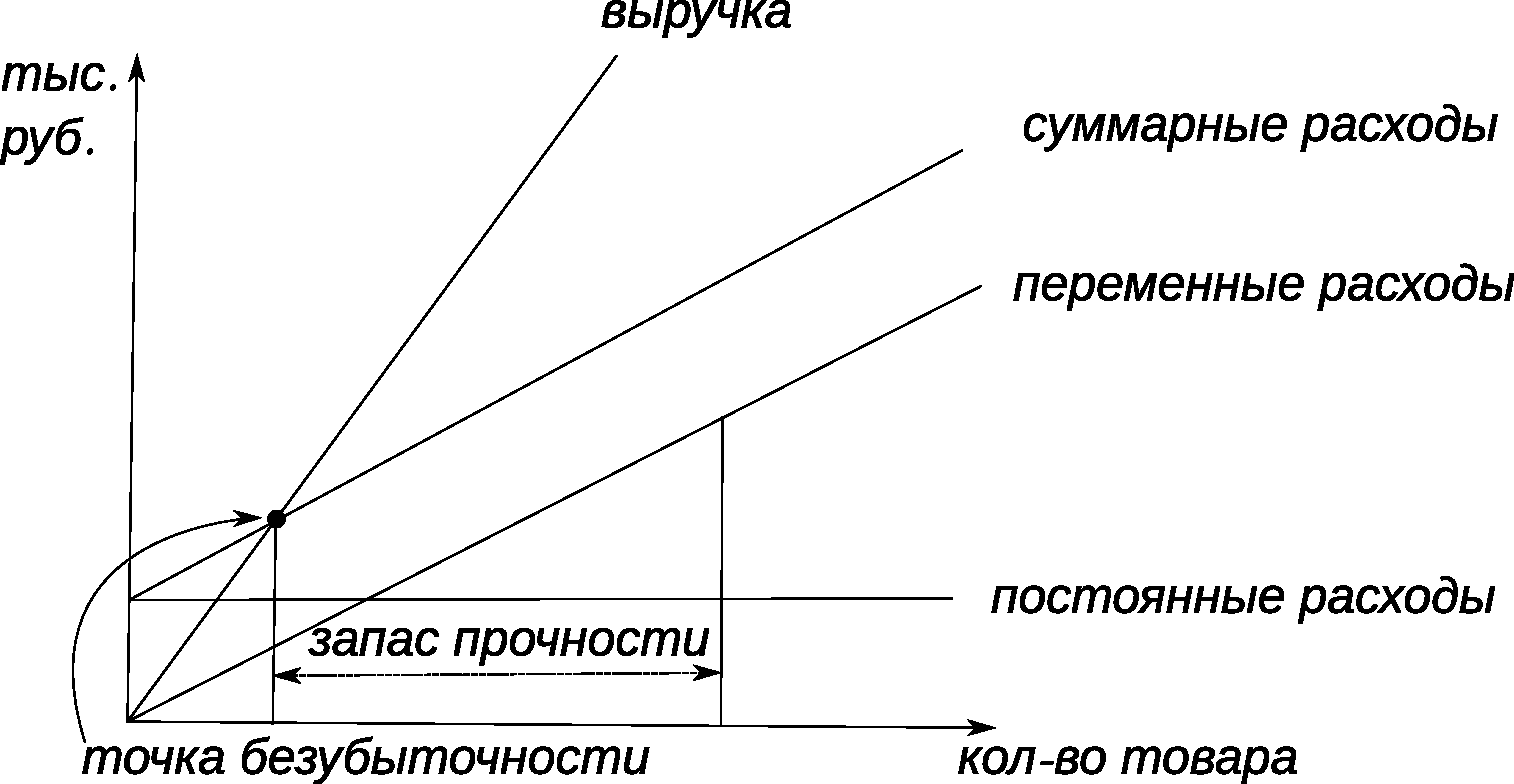
\includegraphics[width=.7\linewidth]{figures/income-goods}
\caption{Доходы и расходы предпринимателя, точка безубыточности, запас прочности.}
\label{fig:income-goods}
\end{figure}


%%%%%%%%%%%%%%
\datee{Feb 19}
Ценообразование 

\begin{tabular}{|c c|}
\hline
Выпуск за месяц & 100 ед \\
Затраты на материалы & 200 р \\
Затраты на ЗП & 150 р \\
Накладные расходы & 10\,000 р \\
Коммерческие расходы & 5\,000 р \\
Продано 80 ед по 550 р & \\
\hline
Определить финальный результат & (два метода) \\
\hline
Метод полного перенесения затрат & \\
Себестоимость & $200 + 150 + \frac{10\,000}{100} = 450$ р \\
Выручка & $80\cdot 550 = 44\,000$ р \\
Себестоимость реального производства & $ 80\cdot 450 = 36\,000$ р \\
Вал. прибыль & $44\,000 - 36\,000 = 8\,000$ \\
Прибыль & $8000 - 5000 = 3000$ \\
\hline
Маржинальный метод & \\
Себест. & $200+150=350$  \\
Выручка & $80\cdot350 = 28000$ \\
Мар. приб. & $44000 - 28000 = 16000$ \\
Валовая прибыль & $16000 - 5000 = 11000$ \\
Прибыль & $11000 - 10000 = 1000$ \\
\hline
\end{tabular}

В первом методе в каждую единицу продукции, в стоимость, включены все затраты, каждый продукт должен моментально окупиться. Но это не позволяет сделать товар особо дешевле. А во втором методе не берутся некоторые расходы в расчет, но это позволяет менять цену гибко, и продавать товар побольше в периоды безденежья людей, а в периоды обилия поднимать. 

\section{Акционерный капитал}
Это важно, потому что подавляющее большинство компаний -- корпорации, акционерные общества. Казалось бы, все гладко и удобно, но есть свои проблемы и злоупотребления. 

Акционерное общество -- предприятие, основной капитал которого разделен на определенное число акций, и участники которого не отвечают по его обязательствам, и несут риск убытков в пределах стоимости принадлежащих им акций. Не отвечают по его обязательствам это значит в противоположность индивидуальным предприятиям и партнерствам, где имущество могут заставить продать, чтобы расплатиться по долгам. В акционерном обществе по-другому распределяется ответственность. Довольно безболезненно позволяет вступать в собственность. Очень легко мобилизовывать средства -- не хватает -- продаем акции и расширяем деятельность. 

Являясь учередитель вносит что-то там сам. Другой вариант, можно не сразу оплачивать, а постепенно пополнять уставной капитал. Когда учередители оплачивают капитал полностью, создается акционерное общество. Но пока нет капитала, нельзя продавать акции. Проблема -- по закону акции лежат мертвым грузом, и через год необходимо что-то там оплачивать. Дальше после того можно расширять деятельность и что-то там делать. Это обговорено изначально должно быть по идее, выпуск дополнительных акций. Эти дополнительные могут распределяться между людьми не учередителями. Акционерное общество перед этим конечно же должно показать свою успешность, чтобы на бирже были акции. Если не будет на бирже, можно как-то там. Это непубличное. Публичное это Initial Public Offering можно одновременно доразмещать по открытой подписке и на бирже. Организация в принципе одинаковая. Берется банк, который берет обязательство реализовать акции акционерного общества, и то же биржа делает, принимая на себя. Чтобы люди хотели это делать, собираются заявки, банк что-то там. Принципы -- эмитент, продающий акции, устанавливает предел, по которому хотят продать акции, дальше через брокеров оставляют люди заявки, сколько хотят купить и по какой цене. И компания должна по идее быстро пройти, потому что эмитенту нужны деньги же. Для скорости можно сузить ценовой диапазон, чтобы инвесторы приобретали уверенность. Работа с инвесторами тяжелая, например если один хочет купить 100\%, а ему дают только 80, то потом на торгах оставшихся 20 он может сказать, а че это я буду втридорого покупать 20, лучше я продам эти 80 и сразу заработаю. В IPO важно еще, что не все компании хотят такое делать, несмотря на то, что деньги быстро получаются, но нужно оплатить посредников, и еще и нужно открытой держать компанию, рассказывать про дела внутри, по семьи глав и так далее. Нашим в России этого не особо хочется. 

Что такое вообще акции. Два вида, обычные и привелегированные (не больше четверти). Разница в рискованности. Обыкновенные считаются самым опасным вложением, потому что нельзя предсказывать даже на месяц, можно и потерять, и приобрести. А люди, которые может быть не захотят участвовать в жизни компании, для них можно выпустить привелегированные акции. По ним дивиденды выплачиваются всегда, кроме ситуации, когда фирма терпит убытки. И дивиденды фиксированы. Но процент у них гораздо меньше, чем на обыкновенных. Еще обычные дают возможность голосовать в делах компании, а привелегированные нет. Есть еще комбинированные варианты, привелегированные с долевым участием. Помимо обычного процента могут выдать дополнительный кусок прибыли компании вдруг, если дела уж очень хороши. 

Акционерные общества могут выпускать облигации, бумаги, подтверждающие, что вы дали взаймы акционерному обществу, и через время можете получить деньги назад и еще +оплату. Долговые отношения считаются более серьезными, и в случае банкротства выплачиваются в первую очередь облигации, потом привелегированные акции, потом обычные. Дальше компания работает, и когда начинает получать прибыль, возникает процесс распределения прибыли. Естественно сначала платят налоги, потом часть прибыли идет в резервный фонд, он важен для возможности акционерного общества производить манипуляции с акциями, затем на расширение производства идет прибыль, затем премии управляющим, а потом из оставшегося дивиденды. Несмотря на то, что уже были уплачены налоги, дивиденды еще раз подвергаются налогообложению, т.к. это типа личная прибыль. Часто мы слышим о капитализации компании, считалось, что можно просто говорить о росте курса акций. Изначально есть номинальная цена акций, а потом они начинают расти. Производственный процесс не затрагивается никак, когда капитализация достигает максимума и падает. Выплачиваются дивиденды, иногда под 50\% даже, и эти деньги выходят из оборота компании. 


Самая главная угроза -- поглощение. Разделение акционеров на мажоритариев и миноритариев (десятые и сотые доли процента). Если кто-то начинает прибирать к рукам акции, и если вдруг у него оказывается контрольный пакет, он может заявить, что вот теперь важное лицо в компании, и хочет сделать что-то с ней. Вывод доходных активов, искусственное банкротство, липовые собрания акционеров, на которых не присутствуют люди многие, и поэтому теряют свои голоса в решении дел компаний. Любая фирма акционерное общество этого всякого боится. Менеджеры кстати могут еще проводить какую-то свою политику, отличную от собственника. Так потому что собственник может не быть спецом в этих делах, а наемникам пофигу на компанию. Эти такие дела менеджеров видны на курсе акций, и когда кто-то поглощает компанию, они вычищают таких. 

\textbf{Англо-Американская модель}

У нас как правило говорится об Англо-Американской модели, в учебниках говорится, что у нас она, и теоретически разбирается она. Признаки 
\begin{itemize}
\item высокое распределение капитала -- много мелких инвесторов
\item они настроены на получение дохода от курсовой разницы, они следят за управленческим аппаратом, следят за менеджерами 
\item основные форма рыночного контроля -- поглощение и слияние 
\item биржа и законодательство страны требует раскрытия финансовой информации, прозрачность нужна для мелких инвесторов 
\item высший орган -- собрание акционеров 
\item из-за распыленности собрание акционеров выбирает совет директоров, есть внутренние директора, которые имеют интерес к компании, и есть внешние, которые арбитры и нацелены на уничтожение злоупотребления управлением 
\end{itemize}

Мелкие акционеры защищены, в основном Америка, Англия, Канада, Австралия, Новая Зеландия, Швеция, Финляндия, Норвегия, Сингапур. 

\textbf{Немецкая модель.} 
\begin{itemize}
\item широкая практика перекрестного владения акциями у компаний одной отрасли, банки и компании так перекрестились, и возникает взаимовыгодное сотрудничество, банк заинтересован в росте акций компании, и дает ей кредиты, а компания, которой дают хорошие кредиты, устойчива 
\item люди не очень стремятся вкладывать в компании, потому что и банки тоже выдают неплохо 
\item активное участие сотрудников в управлении компании, профсоюзы не могут вмешиваться в управление, ибо есть другой механизм. Два органа -- наблюдательный совет (контролирует деятельность, подбирает менеджмент) и ???. Если в компании больше 500 сотрудников, одна треть того может быть своих. 2000 -- половина
\end{itemize}

\textbf{Японская модель}
\begin{itemize}
\item экономику старались демонополизировать, разделили компании семейные, но знакомства и дружба никуда не делись, поэтому компании владеют акциями друг друга. Образовались финансово-промышленные группы, но они уже не семейного плана. 
\item совет директоров играет формальную роль, все директора внутренние, орган подтверждающий просто, а предложения просто идут вертикально снизу вверх 
\end{itemize}

\textbf{Семейная модель}
хз

\textbf{Россия}
\begin{itemize}
\item От Германской модели отличие в банках, заработок на компаниях не велик, мы зарабатываем на людях. 
\item Но общее в том, что собственность на 82\% предприятиях был человек или группа людей, которые управляют компанией безоговорочно. Не работает принцип разделения прав, собственности и контроля. 
\item Среди миноритарных товарищей есть иностранцы, в нашей модели они бесправны. 
\end{itemize}


\datee{Feb 26}

\section{Рынок ценных бумаг}
\subsection{Биржевой рынок}

Рынок ценных бумаг, фондовый рынок. Связаны с акционерным обществом, потому что само оно предполагает существование рынка ценных бумаг, иначе не было бы смысла вообще в бумагах, предлагаемых компаниями. Рынок ценных бумаг, как говорят археологические раскопки, в Месопотамии были таблички с изображениями продавцов. Взаимоотношения между контрагентами стали необходимы, когда усилились финансовые отношения в обществе. При недостатке монет, например, приходилось такими. 
В Италии появляются государственные деньги и облигации со ставкой 5\%, государство занимало. 

Рынок ценных бумаг это система Экономических институтов и механизмов, посредством которых происходит обращение бумаг. Институт это фондовая биржа, но существует и не биржевой. Механизмы это как бумаги попадают, как устанавливается цена их и так далее. Чтобы понять кто действует на рынке, введем понятия. Иммитенты это юр. лица, выпускающие опред. бумаги, и имеющие в связи с этим обязательства. Обычно эти бумаги -- акции и облигации. Выпуская их, они принимают на себя определенные обязанности, в частности выплат процентов или других платежей. Дальше чтобы бумаги находили людей, нужно ввести инвесторов. Это не только юр., но и физ. лица, которые вкладывают деньги в ценные бумаги с целью получения дохода. Институциональные инвесторы это понятие, вводящееся для отделения индивидуальных инвесторов, это пенсионные фонды, страховые компании, банковские структуры. Посредники -- юр. лица, задача которых организовать обращение ценных бумаг. К посредникам относятся брокеры и еще несколько. Брокеры это обычно компании брокерские, скорее не индивидуалы, они заключают сделки по поручениям на средства клиентов. Мы не можем прийти на биржу и просто торговать, нужно обращаться в брокерскую контору, заключается договор, компания открывает счет, вносит деньги (не только заплаченные, но и страхование, доля брокеров итд), брокеры предоставляют информацию людям, она ценная, потому что считается, что биржа это основа вот такого так сказать всего, там аналитика и подобное выше всего. Дальше брокер после введения счета клиента, брокеру можно говорить что когда делать, если разбираешься, либо попросить его самого. Брокеры закупают места на бирже, часто даже аукционные, на крутых биржах места доходят до \$1М. Чем больше объем торговли, тем ниже комиссия, несколько сотен тыс. руб в день это большой. Брокеры платят не только за место, но и за информацию на бирже. То есть по поручениям и за счет клиентов. Дальше из посредников есть дилеры. Дилер совершает сделки за свой счет и покупают бумаги для себя и для продажи третьим лицам. Тут следует обратить внимание на то, что где-то могут написать ``покупают для себя и для своих клиентов'', но это означает именно для продажи клиентам, нельзя как к брокеру прийти и сказать покупай вот это дело. Если ажиотажно возрастает цена чего-то неоправданно, потому что спрос хороший, а предложений мало, биржа должна приостанавливать торги, чтобы успокоить происходящее. Дилеры выступают стабилизаторами рынка, потому что у них запас бумаг и они их предлагают при спросе. Дестабилизация рынка у нас потому что все играют на рост, а не на понижение, это нужно навешивать большой силой банков или хз кого. Должна быть сила, и дилер ей является. Кстати, является ей и спекулянты. Следующий это расчетно-клиринговая палата. Это учереждение банковского типа, осуществляющее обслуживание. Это означает, что Клиринг означает взаимозачет, выплачивается разница, Расчетно это счета. Компания зарабатывает как банг, потому что они берут комиссию и еще потому что лежащие на счетах деньги используются и преумножаются. Главная задача -- организация расчетов и снижение рисков неисполнения дела. Еще один это депозитарий, организация, ведущая счета клиентов, на которых учитываются принадлежащие ценные бумаги, не стоимость, а само наличие. Человек покупает продает, а потом когда он что-то хочет, все высвечивается. Следующий участник это регистратор, ведет реестр владельцев ценных бумаг, это скорее имеющее отношение к эмитенту организация, поскольку заключая договор с регистратором, эмитент может зарегистрировать всех обладателей. Отсюда опасность недобросовестного регистратора, когда он сталкивается с важной информацией, он может продать ее, выдать кому-то собственников акций, чтобы кто-то скупил. Дальше есть джобберы, оценивающие инвестиционные качества ценных бумаг. Их наиболее важная деятельность именно оценка. Важно понять какие все же бумаги продаются теперь, аналитики исследуют рынок, говорят вот вышла компания на рынок, продающая металл, смотрим какие есть конкуренты, насколько она хороша, и говорят какой примерно будет курс акций. Их информация может использоваться не только людьми, но и в основном другие посредники, потому что они не будут изучать сильно глубоко никакие компании. И последние это организаторы торговли, сотрудники биржи, предоставляющие текущую информацию. 

\subsection{Не биржевой рынок}

Дальше надо говорить какие виды в соответствии с какими критериями рынка мы выделяем. Классификация рынков. Обычно выделяют по критерию первые выпуски акций обращаются или уже перепроданные, первичные и вторичные. На одном и том же рынке могут размещать акции новые компании, но это такое понятие чисто теоретическое для того, чтобы были покупатели, нужен вторичный рынок. Более существенное деление -- биржевой и не биржевой. И еще это кассовый срочные. Кассовые расчеты происходят сразу, вы покупаете актив и получаете бумагу. Срочный рынок -- на срок -- говорите, что хотите купить акции за какую-то цену через какое-то время вне зависимости от этого будущего курса. Небиржевой рынок это рынок, в котором ценные бумаги продаются не в пределах биржи. Самый многочисленный, потому что здесь существуют вообще все компании. Всеядность в том, что там не только акции, но и вообще все подряд бумаги. Но и мусор туда не может попасть. Ограничение такое: есть дилеры (они делают погоду на небиржевом рынке, потому что держат бумаги), когда они приобретают бумагу, они не будут брать не пойми что, но поскольку они не рискуют ничем, кроме денег, а биржа репутацией, но если несколько дилеров готовы принимать, то и рынок примет. В этом рынке можно обращаться напрямую к дилерам и говорят, что хотят купить столько-то акций. Проблема небиржевого рынка -- непрозрачность. Небиржевой рынок имеет информационную систему, но она недоступна покупателю, а только брокерам дилерам итд. Часто поэтому называют непрозрачным, несправедливым. Но выход есть через брокера, который видит цену и найдет нужного дилера, возможно комиссия не съест выигрыш. Пусть выходит игрок с колоссальным требованием на покупку, понятно что сразу биржа рванет цену вверх. Даже если он раскидает эти заявки, будет видно, что спрос есть. Такие приколюхи не позволят выгодно купить акции. А такие вложения делают институциональные инвесторы, которым нужно покупать дешевые бумаги. На национальных биржах не будут обращаться акции иностранных компаний, потому что биржа берет большие деньги за включение их в реестр. Биржа всегда такая, потому что она забирает только комиссионные. Иностранные акции покупаются по депозитарной расписке, которая есть аналог акций. Такие расписки это небиржевой рынок, он шире, больше возможностей содержит. В итоге преимущества его в том, что можно из любой точки мира покупать, в любом количестве покупать, информация является неразглашаемой, как на бирже, где можно зафиксировать, и дальше можно купить бумаги компаний еще не обращающихся на бирже. 

Фондовая биржа -- конкретное место, где организована купля-продажа ценных бумаг. Фондовая биржа важна тем, что предоставляет возможность покупать акции первоклассных компаний по низкой цене, чтобы выйти на нее нужно пройти комиссии по листингу (проверяют доход за годы, количество акционеров итд), катировальная (какую катировку поставить, здесь помогают джобберы). Члены биржи могут принимать акции по такой цене, а когда пройдут торги, может измениться цена. Более легкая доступность кредита у финансовых организаций тем, кто на бирже. Более широкие возможности в выпуске облигаций. Больше ценность акций в качестве залога. Торги происходят аукционом, нюансы в том, что если торги идут вяло, заявки накапливаются и потом происходит исполнение. Продавцы хотят продать дороже, а покупатели дешевле, идет торг. Это все отражается в биржевом стакане. 

Дальше поговорим про виды спекуляций. Чисто спекулятивными называют сделки на извлечение выгоды от колебаний цен во времени. Арбитражные сделки приносят прибыль от одновременной купли-продажи на разных рынках. Колебания по месту. Далее про информацию. 

\begin{center}
\begin{tabular}{ c c c c c c c c c c c c }
% высшая цена, низшая за акции
% имя, сокращение имени
% дивиденды, процент от чего-то дивидендов 
% Price to Earnings -- через сколько лет окупится 
% сколько лотов продано, по сколько акций каждый
% цена наивысшая ща день 
% цена наинизшая за день 
% изменение за сутки
Hi & Lo & Stock & Syn & Div & Yet\% & PE & Vol 100s & Hi & Lo & Close & Net Ch. \\
96 & 77 & DuPont & DP & 3.8 & 3.9 & 11 & 13,495 & 98 & 95 & 98 & 2\\
\end{tabular}
\end{center}

Индексы разные бывают, характеризующие рынок, например можно посмотреть на крутые компании и если их акции ухудшаются, значит дело в рынке. Чарлз Доул начал рассчитывать индекс и публиковать в WSJ. 
\begin{enumerate}
\item Первый назывался DJIA (industrial average). Бралось 30 самых крутых промышленных компаний. $p_i$ -- текущая цена акций
$$ I = \frac{\sum_{i=1}^{n} p_i}{N}. $$
Число $N$ связано с дроблением компаний, если сначала в 19 веке было 30, 2002 дал $N=0.1427992$. 
\item S\&P 500 Standard and Put 400 промышленных 20 транспортных 40 коммунальных и 40 финансовых самые стабильные берутся. 
$$ I = \frac{\sum_{i=1}^{n}p_i Q_i}{\sum_{i=1}^{n}p_{Q_i} Q_i}\cdot K, $$
$p_i$ -- текущая цена, $p_{Q_i}$ цена в баз. период, $K=10$.
\item NASDAQ 4862 компании. Как прошлее, но $K=1000$
\item FT-SE100, 100 компаний, такая же ср. арифм. сумма с $K=1000$
\item FT-SE30, 30 компаний, $I_n$ -- темп роста курса,
$$ I = \sqrt[n]{I_1\cdot\ldots\cdot I_n}. $$
\end{enumerate}

Инвестиционные стратегии. Какие бывают акции? Обыкновенные акции делят на первоклассные -- выпускаемые крупными компаниями с безупречной репутацией, по ним выплачиваются регулярные дивиденды, они дорогие, на них можно рассчитывать и как на текущий доход, и на так сказать продажу. Второй вид это доходные -- показывающие высокие дивиденды. Дальше акции роста -- выпускаются быстро растущими компаниями (15\% в год вместо 5\%), дивиденды могут даже вообще не выплачивать. Есть еще циклические акции -- акции компаний, связанных с циклом деловой активности, в период оживления хорошие акции, в период кризиса проседают, это как правило производители оборудования. Противоположные это оборонительные, курс в противоположном направлении к циклу, в кризис поднимаются, это например золотодобывающие компании, потому что в кризис люди вкладываются в золото, далее это коммунальные компании, и лекарственные компании, потому что на последние две вещи кризис не влияет. Последний тип спекулятивный -- нестабильно ведущие себя. И нестабильность привлекательна для рисковых инвесторов, если подгадать на высоком и купить на низком будет ваще круто. 

\textbf{ДЗ} \textit{посмотреть вложения Россиян прошлого года.}

\subsection{Облигации}

Теперь про облигации. Долговые ценные бумаги, по которым инвестор с наступлением срока погашения гарантированно получит денежную сумму, соответствующую номиналу облигации и процент. Характеризует облигацию три параметра -- сама сумма, процент и срок. Процент может быть выплачен единовременно с суммой в конце периода или постепенно. Почему облигации могут быть выгодны. Вот пусть акции уже есть, но компании нужны деньги, компания выпускает облигации. Чем больше выпуск по облигации, тем может хуже быть гарантия. Первыми при банкротстве выплачивают облигации первые. Потом все имущество распродается и идет на другие выпуски облигаций. Дальше, почему облигации, а не кредит. Считается, что облигации дают больший размер, чем может дать банк, затем облигации могут быть на длительные сроки, а кредит не очень. И потом процент по облигациям меньше банковского. Дальше облигации могут выпускаться и без документарной формы, а как запись в депозитарии, что размещено. Доходность, тут надо забежать вперед и поговорить о ставке рефинансирования ЦБ. Кредиты коммерческим банкам выдаются ЦБ, они даются в чрезвычайных ситуациях, когда у банка вдруг не хватает наличности. ЦБ дает под эту ключевую ставку. Эмитенты будут ориентироваться в своей ставке по облигациям на ключевую ставку рефинансирования ЦБ. Государственные и муниципальные облигации. Государство обычно ассоциируется с бюджетом, и если государство хочет заполучить денег, нужны деньги. Есть у государства внешний гос. долг и внутренний. Могут быть как федеральные облигации, так и муниципальные. Государственные облигации самые надежные, но доходность не такая крутая. Единственное только что в нашей истории например в СССР облигации в 82 году выпущены, должны были погашаться в 90, и потом все такое случилось. Еврооблигации теперь. Они называются так потому что появились в Европе в 1963 году, и механизм заложенный тогда применяется много где. Долгосрочные ценные бумаги, которые выпускаются в любой чужой мировой валюте, но не в валюте страны эмитента. Долгосрочность доходит до 40 лет. Краткосрочные в данном случае 1-5 лет. Гос ценные бумаги это до года. Характер выпуска такой. Газпрому нужны были деньги и финансирование, но не в рублях. В долларах решили. Размещать будем не на нашем рынке, привлечем к размещению несколько банков из разных стран. И там их могут приобретать и институциональные, и индивидуальные инвесторы. Но суммы там большие очень могут быть, не менее \$200,000. И еще удобство в том, что по таким облигациям не платится налог. Долгосрочные бумаги всегда обеспечивают хорошую доходность, но краткосрочные. Доходы по гос и муниципальным не подлежат налогообложению, потому что иначе вообще они не нужны. 


\subsection{Производные финансовые инструменты}
\begin{table}
\caption{Доли инвестиций в разных частях мира.}
\label{tab:shares}
\begin{tabular}{l c c c c c c c c}
& Афр. & Азия & Австр. & Евр. & Л.Ам. & Ср.Вост. & С.Ам. & Рос. \\
Акции & 30 & 25 & 35 & 28 & 12 & 25 & 40 & 16 \\
Облигации & 14 & 24 & 19 & 14 & 22 & 19 & 18 & 27 \\
Денежн. активы & 24 & 18 & 16 & 12 & 16 & 14 & 9 & 26 \\
Золото & 1 & 3 & 1 & 2 & 8 & 1 & 1 & 1 \\
Недвиж. & 22 & 23 & 22 & 27 & 17 & 22 & 17 & 20 \\
Предм.роск. & 3 & 2 & 2 & 5 & 11 & 3 & 1 & 3 \\
Частн.акц.кап. & 4 & 4 & 4 & 10 & 9 & 10 & 12 & 7 \\
\end{tabular}
\end{table}
Фьючерсный контракт. Право покупать по какой-то цене вне зависимости от рыночной цены. Но они перешли потом в инструмент игры с ценой. Когда цена нефти падает, падает рубль. Если что-то производится, в основе цены лежит цена производства. Но если спроса нет, все равно цены не будет. И в таком итоге фьючерсные контракты просто инструмент политики и экономики, никакой пользы не дает. 

Инвестирование в драгоценные металлы и сырье. Мы можем инвестировать в слитки золота, серебро, платина, палладий. Можно в монеты, бумажное золото (безличный какой-то счет). Но покупка отжирается на НДС, на доле банка, у которого покупаешь. В итоге нужно, чтобы золото выросло на 20\%, чтобы выиграть. Обезличенный металлический счет, как депозит, только привязан металл. Банк приписывает эквивалент металла данным деньгам, потом цена начинает движение, пусть она поднялась, можно продать золото банку и потом на полученное еще докупить. Подоходный налог не выплачивается, если металл лежит больше трех лет и плюс если общая сумма проданного металла не превышает 250 т.р. в год. Если банк обанкротился, долг не возмещается, страховки нет. 

\datee{Mar 4}

\section{Типы рыночных структур}

Что влияет на то, сколько компаний в отросли может быть. Главное это особенности технологий. Можно выделить 4 структуры. Монополия, Олигополия, Монополистическая конкуренция, Совершенная конкуренция. Совершенная конкуренция~-- понятие из теории, в истории скорее Свободная конкуренция. Начало формирования свободной конкуренции 16 век. В средневековье была цеховая организация, ремесленники объединялись в корпорации, чтобы не было конкуренции, и все в корпорации делали дело очень хорошо, иначе бы выгнали. Потом, следующий период, когда купцы стали под себя ремесло подкупать, с помощью сырья и сбыта, и отсюда зарождение мануфактуры. Мануфактуры были на дотациях, у нас ровно так же, как в Европе. Потом, постепенно увеличивался спрос в силу благосостояния людей, пошло и производство. Оно было мелким, и не могло быть никаким кроме свободной конкуренции. Свободную конкуренцию можно охарактеризовать вот так 
\begin{enumerate}
\item фрагментарная структура спроса и предложения, недостаточность спроса;
\item преобладание мелких и мельчайших фирм;
\item дифференциации продукции почти не было;
\item слабое влияние производителя на торговую марку и на рекламу, производитель сам определял хочет он купить или нет;
\item отсутствие препятствий для внутриотраслевой и межотраслевой конкуренции;
\item невозможность производителю влиять на цены и отсюда отсутствие тенденции к повышению цен;
\item масса прибыли производителя зависела от его способности снижать издержки, нельзя было наращивать производство и продавать больше, никто не покупал. 
\end{enumerate}

Этот период до кризиса 1873 года, который послужил толчком к процессу концентрации производства. Это пятый или шестой кризис, с которым столкнулись хозяйства. Этот период уже можно назвать периодом господства монополии. Производство увеличивало объем, и компании получали все большую рыночную долю. 1884 году доли 10\% было сложно достичь, а в 1914 -- 46\%. Но при чем здесь кризис? Ну, концентрация производства это огромный капитал, который позволяет увеличивать активы, а акционерные общества тогда работали, и они собирали большие капиталы. Потом еще кредиты, банковская система сильно развертывалась тогда, это был вообще период дикого капитализма и банковского диктата. Тогда банков было много, они часто разорялись, а никакой страховки не было совершенно, деньги просто исчезали. Мелкие банки из-за конкуренции шли на рисковые вещи и разорялись, а большие компании переманивали к себе, и все больше диктовали. Кроме того, крупные компании имели большие резервы и могли себе позволить сильно понижать цены. Монополия это фирма, имеющая настолько высокую долю на рынке товара, не имеющего заменителей, что это позволяет ограничивать объем производства и влиять на цену. Монополист сам цену устанавливает, для него спрос это по сути величина уже вторая. Нужно еще заметить. Монополия сама складывалась редко, нужны были толчки. Протекционизм. В Америке была сильная конкуренция с Англией, потом гражданская война, экономически было то, что Юг использовал рабов, издержек было меньше. Для реализации нужен был рынок. А север был промышленный, и там не было у Америки преимуществ перед Англией. В условиях протекционизма от внешнего мира строились предприятия, которые потом становились монополиями. Еще было лоббирование. Америка единственная страна, где железные дороги не были монопольными, но потом в результате лоббирования они протолкнули идею, что ЖД бизнес невозможен без монополии, но с такими вещами боролось антимонопольное что-то. В 1890 году первый закон антимонопольный был издан. Дальше следующий путь отсечения конкурентов это патенты, которые скупаются, и другие производители в результате не просто не могут конкретный товар производить, но и близко похожие. Монополии создавали непреодолимые барьеры для входа в отрасль. Две точки зрения: монополия уже монополия, она не стремится к совершенствованию; но у монополии есть капиталы, они могут сильно вкладывать в разработки, а малые компании сидят вечно на кредитах и естественно не могут себе позволять что-либо. Еще один интересный факт: текстильная промышленность не была монополизирована, хоть и концентрация производства была мощная. Причина была в спросе, просто не было спроса на текстиль. А вот если бы это было какое-то оборудование для фабрик, например, тогда монополизация была бы крута. Теперь, монополист же понимает, что большая цена это отсечение кучи потребителя, поэтому он думает как продать людям за максимальную для них цену, это политика ценовой дискриминации. Это назначение разных цен для разных категорий потребителя в зависимости от характера их спроса, от того, сколько действительно человек может заплатить. На деле разделяют на магазины для богатых и обычные магазины, их посетители никак не будут пересекаться. Еще бывают льготы для пенсионеров / студентов. Потом бывает разделение по объему товара. Вообще, монополисту круто, потому что он может регулировать малыми изменениями большой цены, и изменения объемов будут сильно менять заработанные с продажи всего деньги, как показано на рис.~\ref{fig:price-quantity}.

\begin{figure}
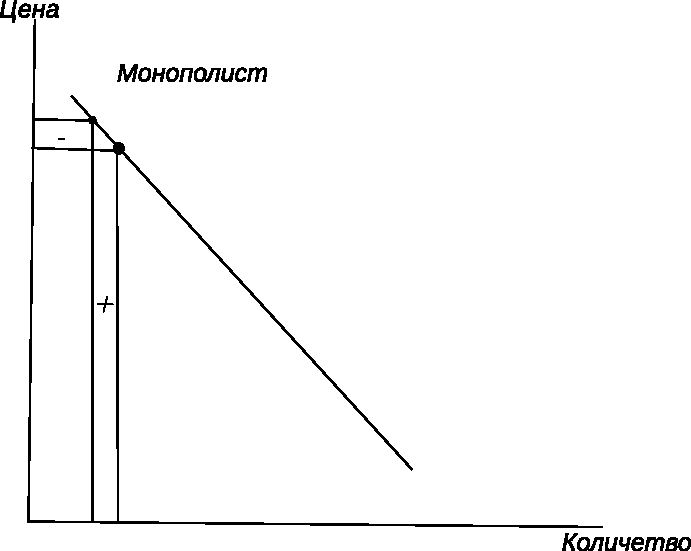
\includegraphics[width=.5\linewidth]{figures/price-quantity}
\caption{Ценовая политика монополиста.}
\label{fig:price-quantity}
\end{figure}

Теперь поговорим о естественной монополии. Иногда барьеры для входа в отрасль имеют не искусственный характер. Тогда возникает естественная монополия, когда наличие большого числа производителей снижает эффективность. Например, в нефтяной отрасли нужны трубы, и на них нужны затраты и на создание, и на поддержание. 

\begin{figure}
\includegraphics[width=.5\linewidth]{figures/natural-monopoly}
\caption{Причина естественной монополии -- высокие затраты при малом количестве производства.}
\label{fig:natural-monopoly}
\end{figure}

Американские товарищи все врем законодательно боролись с монополией. Возникали различные взаимоотношения между копаниями для борьбы с таким. Олигополия -- существование нескольких ведущих крупных фирм, которые опираются на поведение друг друга, они обязательно должны отслеживать друг друга поведение. Признаки рынка: однородный или дифференцированный продукт (нефть или холодильники); высокие барьеры вхождения. Самая важная причина образования -- технологическая. Технологии приводят к существованию минимального эффективного масштаба. Вторая причина это конечно колоссальные затраты. Например автомобильное производство. Самые сильные волны слияния: когда-то, после кризиса, 1960, и сейчас. 

\begin{figure}
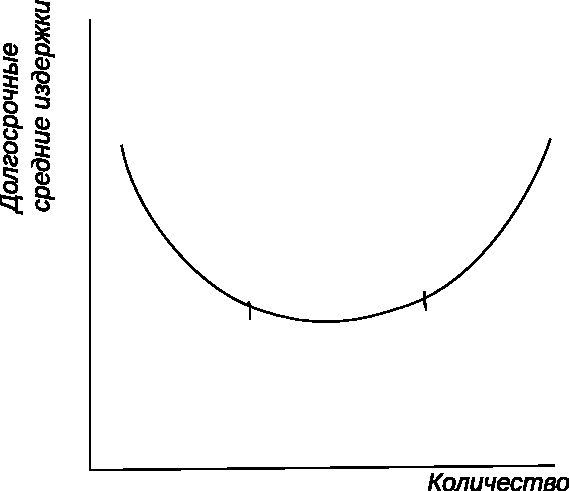
\includegraphics[width=.5\linewidth]{figures/oligopoly}
\caption{Причина олигополии -- высокие затраты при малом или при большом количестве производства.}
\label{fig:oligopoly}
\end{figure}

Поведение монополиста. Нескоординированная олигополия -- один чел понижает цену, и думает, что другие не сделают, а они делают естественно, и вся отрасль просто проигрывает. Лидерство в ценах -- одна, самая продвинутая фирма меняет цену, потом товарищи тоже делают так, если согласны, или же остаются как были. И тогда этот лидер не идет дальше не реализует свои планы. Картели были еще, они делили рынок и устанавливали разные цены в разных местах, ограничивали срок службы продукции итд. Вертикально интегрированные структуры. Например для бетона нужны карьеры, а карьерный бизнес довольно монопольным может оказаться. И тогда делающие бетон товарищи интегрируются с карьерными, ну или последние с первыми. Олигополия может понижать цену, иногда даже во много раз. Крупное производства, сеть сбыта, сырье -- три важные вещи для производства, если они есть, ты засел просто на века. Еще интеграция позволяет убыточное за счет прибыльного компенсировать. 

Монополистическая конкуренция. Признаки рынка. Большое число мелких производителей, Дифференциация продукции, Незначительные барьеры для вхождения. Дифференциация это создание реальных или мнимых различий в товаре, обеспечивающая некоторую мнимую монопольную власть. Монопольную власть дает приверженность. Большие успехи рекламы приводят к спросу, нужно больше производить, но спрос потом спадет, а производственные мощности простаивают. Если хочешь войти в отрасль с крупными людьми, нужно выбрать какую-то нишу и ее толкать. Но там сложно выбрать, трудно удержать, и необходимо учитывать спрос, приходится часто выходить на мировой рынок, где сильная конкуренция. 

Коэффициент концентрации. Индекс Герфиндаля. $q$ -- доля фирмы на рынке. 
$$
G = \sum_i q_i^2  
$$
$<400$ свободная конкуренция. 400-1000 -- монопольная конкуренция. 1000-3000 олигополия. $>3000$ -- монополия. 
















\end{document}
